% future_developements.tex

We have stepped through, in detail, the low-mass \ac{CBC} pipeline, and we have described how this was used to obtain search results. We now conclude by briefly presenting some future developements for the pipeline.

\section{Gating}

In chapter \ref{ch:s6_results} we saw the effects a loud transient --- the spike glitch --- had on the matched filter. We dealt with the spike glitch by adding a category 3 veto around the time of the glitch. Due to the ringing of the filter we had to add a $\pm 8\,$s padding to the glitch. However, as can be seen in figure \ref{fig:spike_glitch-cbc_response}, triggers can be last for several tens of seconds after the glitch; this duration increases with the size of the glitch.

Another possiblity is to remove the glitch \emph{prior} to match filtering. We can do this by applying a Tukey window to the data stream to ramp the output down to $0$ at the time of the glitch. We call this ``gating." Figure \ref{fig:gating-time_series} shows a time series in which a spike-glitch occurred with a gate applied.  In \ref{fig:gating-time_series-gated} the window that is applied can be seen. We must ramp the data down (in this case, by using the first half cycle of a cosine) so as not to introduce ringing at the point the window turns on, and we must do the same after the glitch to ramp the data back up. In this manner we can cleanly remove the glitch from the data: compare the Omega scans in figure \ref{fig:gating-omega_scans} with the glitch in to the scan with the glitch out.

Zeroing out the data around the glitch does mean that we will slightly underestimate the \ac{PSD}. However, if the gated data is only a few seconds out of an entire analaysis chunk, the effect should be small. It may also be possible to correct for the zeroed out data by taking the average power across the segment, then add a correction factor. Even if we add a correction factor to the \ac{PSD}, we should probably limit the amount of time that is gated in an analysis chunk. The upper limit on how much time can gated in a chunk requires more study.

Knowing what to gate also needs study. In the case of the spike glitch, we could not find the cause, as we could not correlate it with any ``safe" channel. We got around this difficulty by applying the \ac{SNR} $> 250$ flag at CAT3, which allowed us to check the results at CAT2 to ensure we did not accidently veto a loud \ac{GW} triggers. Since gating involves removing the glitch before filtering, we would not have that luxury, unless we were to match filter the data multiple times. Another possibility is to establish a \ac{SNR} for which burst searches do as-good-as \ac{CBC} searches at finding \ac{GW} signals. We would then remove any trigger that exceeded that threshold, leaving it to the burst, or a mixed burst-\ac{CBC} search to find loud triggers. Finding that threshold, and determining the safety of such a scheme, is yet to be done.

\begin{figure}[p]
\center
\subfigure[Raw time series.]{\label{fig:gating-time_series-raw}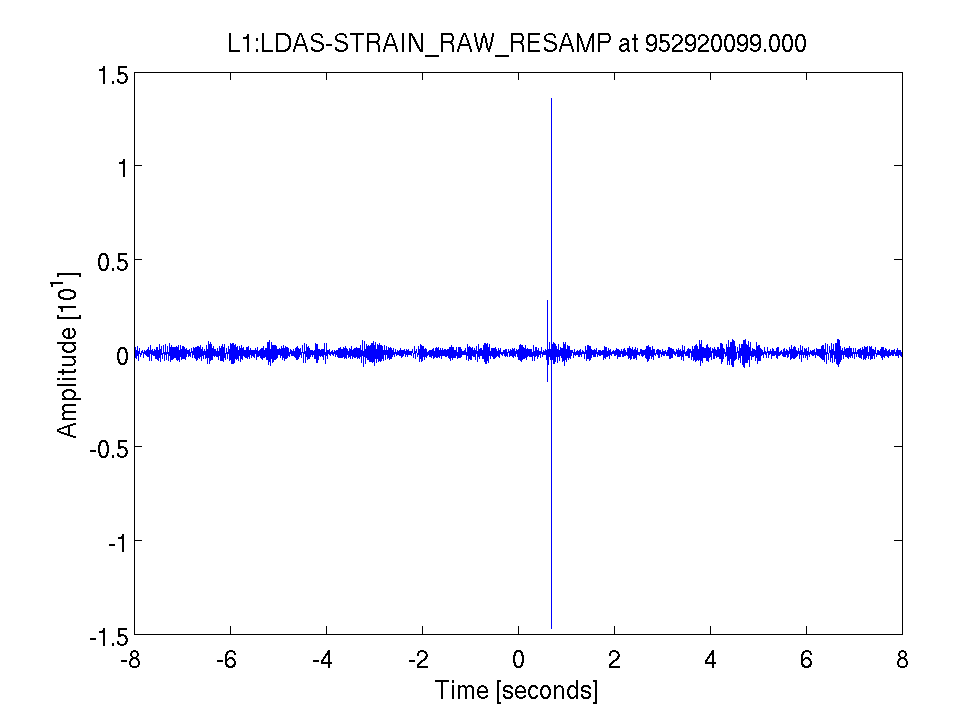
\includegraphics[width=4.75in]{figures/gating/time_series-spike.png}}
\subfigure[Gated time series.]{\label{fig:gating-time_series-gated}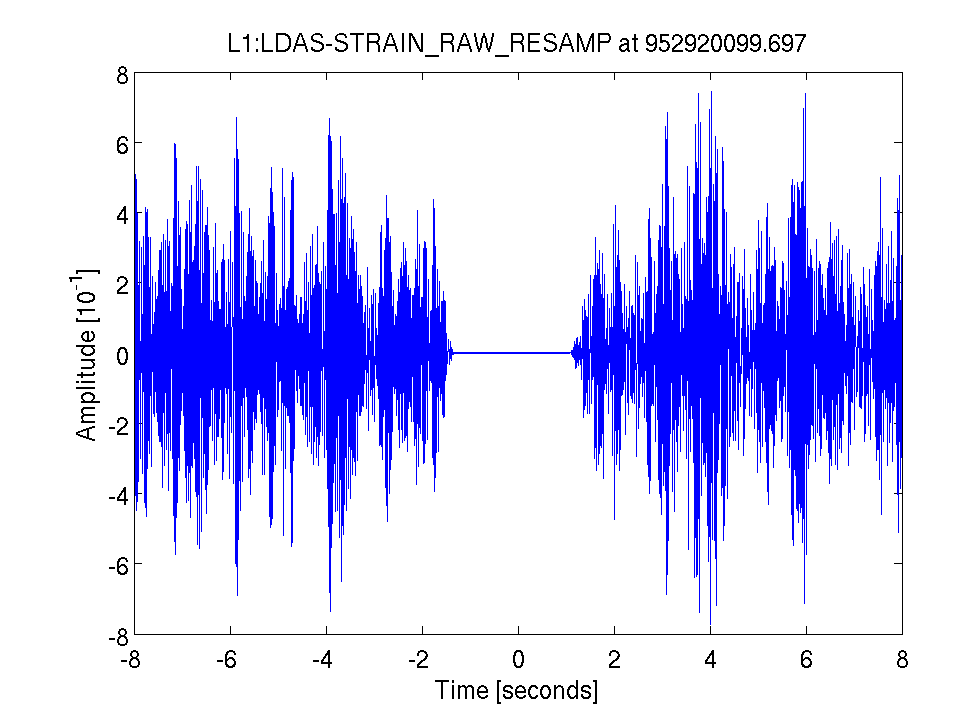
\includegraphics[width=4.75in]{figures/gating/time_series-gated.png}}
\caption{Raw and gated time series of a L1 spike glitch that occurred during \ac{S6}. In the raw time series (top) we can see that this was actually two glitches in quick succession. For this reason, the gate was chosen to be $\pm1.5s$ around the larger glitch. The effect of the ramping down of the Tukey window can be seen in the gated time-series.}
\label{fig:gating-time_series}
\end{figure}

\begin{figure}[p]
\center
\subfigure[Scan with glitch in.]{\label{fig:gating-omega_scan-raw}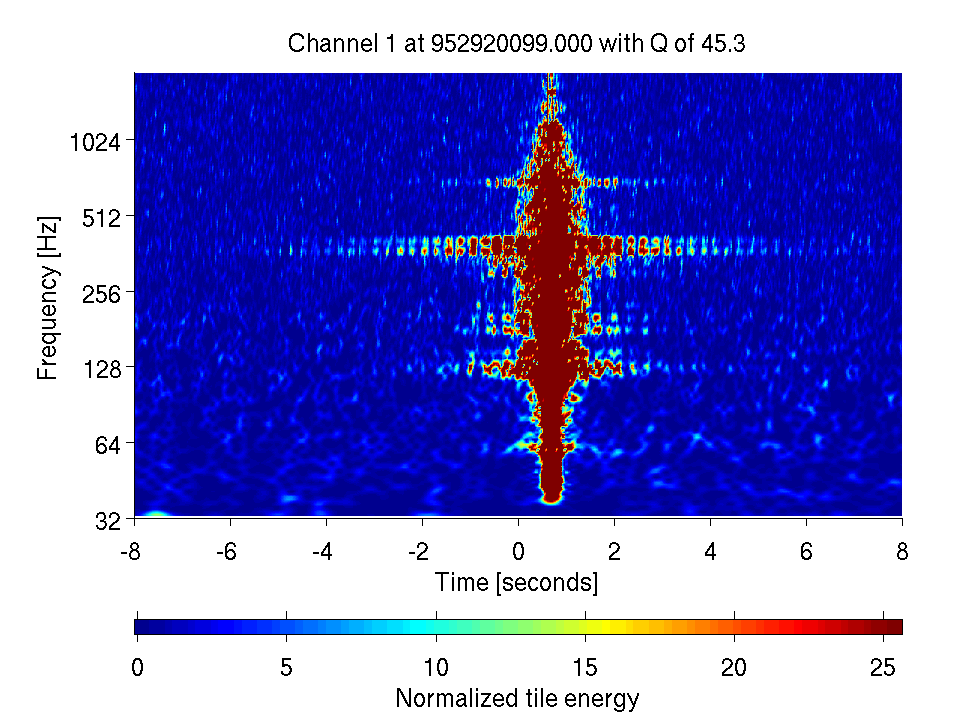
\includegraphics[width=4.75in]{figures/gating/omega_scan-spike.png}}
\subfigure[Scan with gate.]{\label{fig:gating-omega_scan-gated}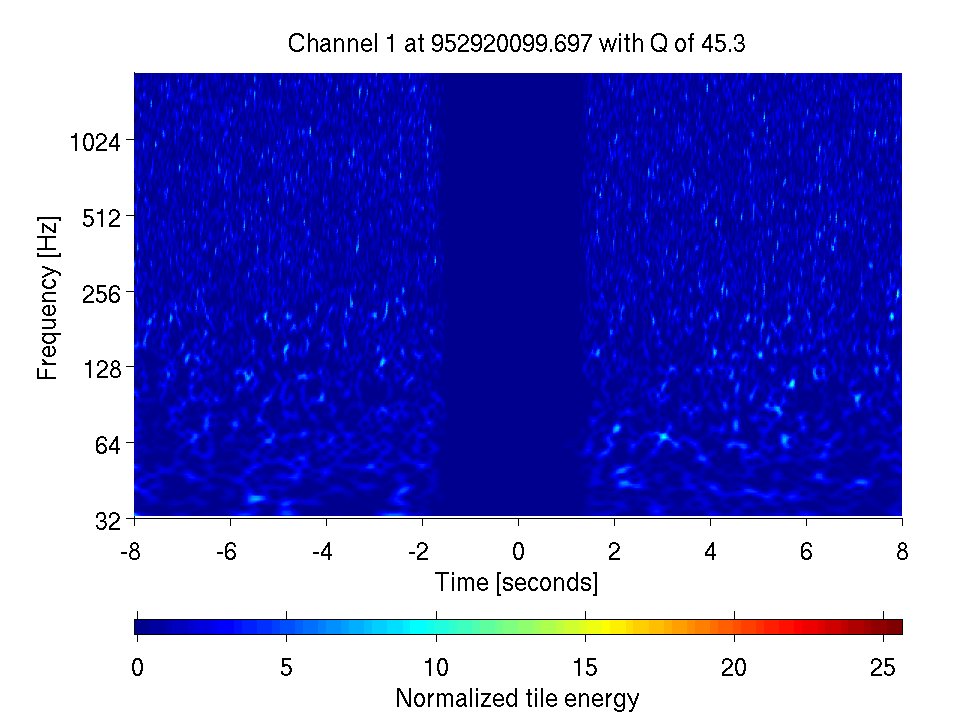
\includegraphics[width=4.75in]{figures/gating/omega_scan-gated.png}}
\caption{Omega scan of the spike glitch shown in figure \ref{fig:gating-time_series}. The top plot shows the scan with the glitch in the data; the bottom plot shows the scan with the glitch removed. Omega applies a whitening filter when these scans are generated. The ringing of the filter is evident in the top plot. With the glitch gated, we see that there is no ringing.}
\label{fig:gating-omega_scans}
\end{figure}

\section{Single Stage Pipeline and Updates to Pipedown}

Using a two stage-pipeline, as presented in chapter \ref{ch:ihope_pipeline}, makes it difficult to followup triggers, and to do things such as perform more slides, as dicussed in chapter \ref{ch:s6_results}. \ac{HIPE} was developed to have two stages in order to save on the computational cost of calculating $\chi^2$. This was done several years ago. Since then, advancements in computing speed have made it possible to use a \emph{single-stage} pipeline. In this, $\chi^2$ is calculated at first inspiral, and so no second stage is needed. Having such a pipeline would make it far simplier to followup triggers and to know how they evolve through the pipeline.

As mentioned in \ref{ch:s6_results} a prototype single-stage pipeline already exists. Some updates need to be made to Pipedown to be able to use this pipeline, however, as some of the programs rely on conventions of the current \ac{HIPE} pipeline. Of note: in the singe-stage pipeline, \verb|lalapps_thinca| is replaced by an updated verison, \verb|ligolw_thinca|, which natively makes use of the Coinc and Experiment tables discussed in chapter \ref{ch:ihope_pipeline}. It also performs linear slides as opposed to slides on a ring. This removes the need for \verb|ligolw_thinca_to_coinc| in Pipedown.

A few other improvements are also planned for Pipedown. As mentioned in Chapter \ref{ch:ihope_pipeline}, multiple veto categories can be stored in a single database. Pipedown currently does not take advantage of this. As part of the switch to a single-stage pipeline, we plan to add a program to Pipedown to apply vetoes in the database, so as not to have to run \verb|ligolw_thinca| multiple times. Also, a number of programs in Pipedown cannot read data from multiple databases. This makes it difficult to combine results from multiple runs. Reading from multiple databases will require a slight update to the \verb|experiment| table. Namely, we plan to replace the \verb|gps_start| and \verb|gps_stop| columns with a \verb|segment_def_id| column. This would point to a list of segments in the \verb|segment| and \verb|segment_definer| tables that give the analyzed time covered by the database.

Pipedown can also be greatly simplified. Currently, it has to create intermediate databases that separately store injection data from each of the runs. These \verb|RAW| databases lack much information, such as the vetoes applied and the livetime. This is done so as to limit the size of the xml files that need to be extracted for \verb|lalapps_inspinjfind|. Since clustering is done on these intermediate databases it makes it difficult to test new statistics. If one wants to cluster with the new statistic, they must re-run clustering on all of the individual \verb|RAW| databases, carry out injection-finding, create a new final database, and re-compute the livetime. If \verb|lalapps_inspinjfind| could read databases instead, all of the injection runs could be added to the \verb|FULL_DATA RAW| database at the outset, greatly simplifying the pipeline and the ability to test new statistics. Work on this is planned. Along with this update to the injection finding program, we plan to implement more sophisticated injection finding techniques, such as using ethinca windows.

Finally, note that out of all the tables Pipedown makes use of, only the \verb|coinc_inspiral| and \verb|sngl_inspiral| are specific to the low-mass \ac{CBC} search. All mappings between the Experiment --- which can be used for any search --- and the other Coinc tables are based on the \verb|coinc_event_id|. Thus, if another search uses tables that are equivalent to \verb|sngl_inspiral| and \verb|coinc_inspiral| tables, all these tables need are a \verb|event_id| column and a \verb|coinc_event_id| column and they can make use of the same architecture. All the programs run by Pipedown could then run on any search; we just need to swap out pointers to the \verb|coinc_inspiral| and \verb|sngl_inspiral| table for more generic names that could be set in the configuration file. We have done just that for the \ac{CBC} group's \emph{ringdown} search. This search looks for \acp{GW} emitted by black holes after they coalesce and are ``ringing down." This search stores its single-\ac{IFO} in a \verb|sngl_ringdown| table and its coincident data in a \verb|coinc_ringdown| table, which have \verb|event_id| and \verb|coinc_event_id| columns, respectively. A prototype of Pipedown has been developed that takes the table-names from the configuration file. By simply changing the parameters in the configuration file, we have been able to run Pipedown on this search. This update is currently being tested.

%\section{Calculating False Alarm Rates from Single IFO Distributions}
%
%As we saw in chapter \ref{ch:s6_results}, the presence of a signal in the data --- in our case, it was a blind injection --- can alter the background estimation for that trigger. We saw why this happens in equation \ref{eqn:slideTerms} in Chapter \ref{ch:far}: if the probability is high that a signal exists in the data, it mixes with the noise triggers to increase the background estimate. This problem is compounded if there are multiple signals in the data, as may be the case in advanced \ac{LIGO}.
%
%One possibility to deal with this is to remove the single-\ac{IFO} triggers associated with a given foreground coincidence from the slides when computing the false alarm rate for that trigger. We pioneered this in \ac{S6} when we estimated the false alarm rate for the blind injection. However, concerns arose that if the blind injection were from noise, we would underestimate its \ac{FAR}.
%
%Another possibility is suggested by equation \ref{eqn:exptd_slid_coincs}. If we fit a probability distribution in new \ac{SNR} of the single-\ac{IFO} triggers (before coincidence testing), we could get a false alarm rate by performing the integral in \ref{eqn:exptd_slid_coincs}, with the \ac{GW} term set to zero. Although a signal may exist in the data, the fit would be less suscepitible to its influence than time slides, since, persumably, the number of signals would be far less than the number of noise triggers. The difficulty in this method is establishing what distribution to use. Although new \ac{SNR} removes most of the non-Gaussian tail, it is not clear that resulting distribution should be $\chi^2$ distributed with two degrees of freedom. Further, a 

\section{Conclusion}

The data-analysis methods, pipeline, and search results presented in this thesis are the result of years of work by a number of people throughout the \ac{LSC} and the Virgo Collaboration. Although no gravitational-waves have been detected as of yet, injection studies, comparisons of our upper-limits to astrophysical predictions, and the result of the \ac{S6} blind injection challenge have made us confident that we will be able to detect when advanced \ac{LIGO} and Virgo come online. The work to build advanced \ac{LIGO} is currently underway. When it is finished it will present new challenges to our data analysis pipeline, some of which are outlined here. In the coming years we will continue to improve and refine our analysis techniques to meet those challenges, so that, when an event happens, we will detect it.
